%! Author = Len Washington III
%! Date = 11/05/2023

% Preamble
\documentclass[24]{cs430lecture}

% Packages

% Document
\begin{document}

%<*Lecture-Activity-24>
\maketitle
\openingquestions

\begin{enumerate}
    \item Give an example NOT discussed in the video lecture of a problem that can be represented by a graph.
	\item If there is a path in a graph from a vertex back to itself, that is called a
	\underline{~~~~~~~~~~~~~~~~~~~~}.
	\item Which representation of a graph, adjacency-list and adjacency-matrix, usually uses more memory and why?
\end{enumerate}

\section{Graphs}\label{sec:graphs}
\begin{enumerate}
    \item Draw the graph:
	A directed graph $G=(V,E)$ where $V=\{ 1, 2, 3, 4, 5, 6 \}$ and $E=\{ (1,2), (2,2), (2,4), (2,5), (4,1), (4,5), (5,4), (6,3) \}$.
	What is the edge $(2,2)$ called?
	\item Draw the graph:
	An undirected graph $G=(V,E)$ where $V=\{ 1, 2, 3, 4, 5, 6 \}$ and $E=\left\{ \{1,2\}, \{ 1, 5\}, \{ 2, 5\}, \{ 3, 4\} \right\}$.
	What is vertex $4$ called?
	What is the difference about how an edge set $E$ is denoted for an undirected graph?
	Are self-loops allowed in an undirected graph?
	\item Define these terms:
	\begin{itemize}
		\item Vertex $v$ is adjacent to vertex $u$ in an undirected graph.
		\item Vertex $v$ is adjacent to vertex $u$ in a directed graph.
		\item The degree of a vertex in an undirected graph.
		\item The degree of a vertex in a directed graph.
		\item A path in an undirected graph.
		\item A path in a directed graph.
		\item The length of a path.
		\item $v$ is reachable from $u$.
		\item A simple path.
		\item A cycle in an undirected graph.
		What about a simple cycle?
		\item A cycle in a directed graph.
		What about a simple cycle?
		\item Acyclic graph.
		\item Connected undirected graph.
		\item Connected directed graph.
		\item Bipartite Graph.
	\end{itemize}
\end{enumerate}

\section{Graph Implementations}\label{sec:graph-implementations}
\begin{enumerate}[start=4]
    \item What is the adjacency list implementation of these two graphs?

	\begin{minipage}{0.5\textwidth}
		\begin{figure}[H]
			\centering
			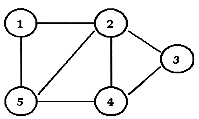
\includegraphics[width=\textwidth]{24.1}
			\label{fig:24.1}
		\end{figure}
	\end{minipage}\begin{minipage}{0.5\textwidth}
		\begin{figure}[H]
			\centering
			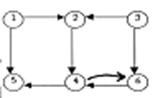
\includegraphics[width=\textwidth]{24.2}
			\label{fig:24.2}
		\end{figure}
	\end{minipage}
	\item What is the adjacency matrix implementation of the above two graphs?
	\item How do the two implementations handle a weighted graph?
	\item Two different representations of the graph data structure are discussed in the book, adjacency-list and adjacency-matrix.
	Please briefly discuss the runtime (in terms of $|V|$ and $|E$ of these graph operations/algorithms using each implementation.)
	Assume vertices are labeled as integers.
	\begin{itemize}
		\item What is the worst-case big-O runtime for checking to see if an edge from vertex $u$ to vertex $v$ exists?
		\item How long does it take to compute the out-degree of every vertex of a directed graph?
		\item How long does it take to compute the in-degree of every vertex of a directed graph?
	\end{itemize}
\end{enumerate}

\section{Graph Traversals}\label{sec:graph-traversals}
A way to search/visit all the vertices in a graph.
There is not a unique answer usually.
\begin{itemize}
	\item Undirected graph - if connected, all vertices will be visited.
	\item Directed graph - Must be strongly connected to be able to visit all vertices.
\end{itemize}

Breadth first - visit vertices one edge from a given (or random) source, two edges from source, etc.
Uses a queue and some way to make a vertex (white initially, gray when first visited and put in queue, black when out of queue),
label a vertex how far from the source, and label a vertex with how its predecessor vertex was during the traversal.

\begin{enumerate}[start=8]
    \item Perform a breadth first search on this graph.
	\begin{figure}[H]
		\centering
		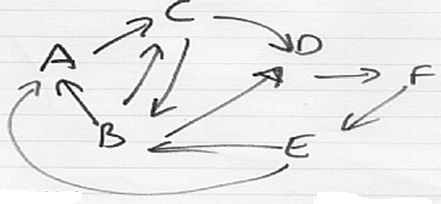
\includegraphics[width=\textwidth]{24.3}
		\label{fig:24.3}
	\end{figure}
\end{enumerate}

\begin{algorithm}[H]
	\caption{Breadth-First Search for Graphs}\label{alg:graph-bfs}
	\begin{algorithmic}[1]
	\Function{BFS}{$G$, $s$}
		\ForAll{vertex $u\in V[G] - \{s\}$}
			\State \Call{Color}{$u$} $\gets$ WHITE	\Comment{Unvisited}
			\State $d[u]\gets\infty$
			\State $\pi[u] \gets$ NIL
		\EndFor
		\State \Call{Color}{$s$} $\gets$ GRAY		\Comment{First time seen, put in queue}
		\State $d[s]\gets0$
		\State $\pi[s]\gets$ NIL
		\State $Q\gets\emptyset$
		\State \Call{Enqueue}{$Q$, $s$}
	\While{$Q\neq\emptyset$}
		\State $u\gets\Call{Dequeue}{Q}$
		\ForAll{$v\in\Call{Adj}{u}$}
			\If{$\Call{Color}{v} == $ WHITE}
				\State $\Call{Color}{v}\gets$ GRAY
				\State $d[v]\gets d[u] + 1$
				\State $\pi[v]\gets u$
				\State \Call{Enqueue}{$Q$, $v$}
			\EndIf
		\EndFor
		\State $\Call{Color}{u}\gets$ BLACK			\Comment{Last time seen, out of queue}
	\EndWhile
	\EndFunction
	\end{algorithmic}
\end{algorithm}
%</Lecture-Activity-24>

\end{document}